\documentclass[a4paper,14pt]{article}

\usepackage{comment} % Para comentar várias linhas ao mesmo tempo

%matemática
\usepackage{amsmath}
\usepackage{amssymb}

%diagramação
\usepackage{extsizes}
\everymath{\displaystyle}
\usepackage{geometry}
\usepackage{fancyhdr}
\usepackage{multicol}
\usepackage{graphicx}
\usepackage[brazil]{babel}
\usepackage[shortlabels]{enumitem}
\usepackage{cancel}
\usepackage{textcomp}
\usepackage{tcolorbox}

%tabelas
\usepackage{array} % Para melhor formatação de tabelas
\usepackage{longtable}
\usepackage{booktabs}  % Para linhas horizontais mais bonitas
\usepackage{float}   % Para usar o modificador [H]
\usepackage{caption} % Para usar legendas em tabelas
\usepackage{wrapfig} % Para usar tabelas e figuras flutuantes
\usepackage{xcolor} % Para cores do fundo de tabelas
\usepackage{colortbl} % Para cores do fundo de tabelas

%tikzpicture
\begin{comment}
	\usepackage{tikz}
	\usepackage{scalerel}
	\usepackage{pict2e}
	\usepackage{tkz-euclide}
	\usetikzlibrary{calc}
	\usetikzlibrary{patterns,arrows.meta}
	\usetikzlibrary{shadows}
	\usetikzlibrary{external}
\end{comment}


%pgfplots
\usepackage{pgfplots}
\pgfplotsset{compat=newest}
\usepgfplotslibrary{statistics}
\usepgfplotslibrary{fillbetween}

%colours
\usepackage{xcolor}



\columnsep=2cm
\hoffset=0cm
\textwidth=8cm
\setlength{\columnseprule}{.1pt}
\setlength{\columnsep}{2cm}
\renewcommand{\headrulewidth}{0pt}
\geometry{top=1in, bottom=1in, left=0.7in, right=0.5in}

\pagestyle{fancy}
\fancyhf{}
\fancyfoot[C]{\thepage}

\begin{document}
	
	\noindent\textbf{6FMA112 - Matemática} 
	
	\begin{center}Princípio multiplicativo (Versão estudante)
	\end{center}
	
	\noindent\textbf{Nome:} \underline{\hspace{10cm}}
	\noindent\textbf{Data:} \underline{\hspace{4cm}}
	
	%\section*{Questões de Matemática}
	
	\begin{multicols}{2}
		\noindent \begin{itemize} 
		\item \textbf{Princípio multiplicativo:} sempre que tivermos possibilidades de escolhas dependentes, ou seja, sempre que duas possibilidades diferentes unidas gerem resultados finais diferentes, iremos \textbf{multiplicar} a quantidade de possibilidades para cada escolha. Esse processo é caracterizado pela conjunção \textbf{e}.
		\end{itemize}
		\noindent\textsubscript{-----------------------------------------------------------------------}
		\begin{enumerate} 
			\item Jorge adora fazer trilhas. Em um fim de semana, ele visitou uma reserva que tem um mirante e uma cachoeira, ambos acessados por trilhas. Para chegar ao mirante a partir da entrada da reserva há 5 trilhas, e do mirante à cachoeira há 4 trilhas. De quantas maneiras diferentes Jorge pode ir da entrada da reserva até o mirante e depois ir à cachoeira? \\\\\\\\\\\\\\\\\\\\\\\\
			\item Kátia adora usar vestidos. Durante o inverno, ela separa 4 casacos que combinam com qualquer um de seus 6 vestidos. De quantas maneiras diferentes Kátia pode usar a combinação de um vestido e um casaco no inverno? \\\\\\\\\\\\\\\\\\\\\\\\
			\item Marcelo, Michele e seus 3 filhos vão fazer uma viagem de carro. Como seus filhos ainda são pequenos, devem ir no banco de trás, e Marcelo ou Michele podem dirigir. Sabendo que no carro há 2 lugares na frente e 3 atrás, de quantas maneiras a família pode se acomodar no carro? \\\\\\\\\\\\
			\item As placas de automóveis de certo país são compostas por 4 letras e 3 algarismos, nesta ordem, podendo ou não ser repetidos. Quantas placas diferentes existem somente com as letras $A, B, C$ e $D$ e os algarismos 1, 2 e 3? \columnbreak
			\item Uma rede de $fast-food$ oferece a seus clientes a opção de escolher cada ingrediente de seus lanches. O cliente precisa, necessariamente, escolher um ingrediente dentre cada uma das categorias: pão, queijo, legume, hambúrguer e molho.
			\begin{enumerate}[a)]
				\item Para cada categoria, dê um número de opções de ingredientes disponíveis na rede de $fast-food$.
				\begin{itemize}
					\item pão: $\underline{~~~~~~}$ opções;
					\item queijo: $\underline{~~~~~~}$ opções;
					\item legume: $\underline{~~~~~~}$ opções;
					\item hambúrguer: $\underline{~~~~~~}$ opções;
					\item molho: $\underline{~~~~~~}$ opções;
				\end{itemize}
				\item Agora, responda: quantas combinações de lanches podem ser feitas nesta rede de $fast-food$? \newpage
			\end{enumerate}
			%5 a 8
			\item A família Toledo vai sair de férias e, antes de chegar a seu destino, deixa seu cachorro no sítio de um amigo na cidade Estrela, situada entre a casa deles - na cidade Sol - e a cidade Diamante, onde eles passarão as férias. Há 3 estradas que vão de Sol a Estrela e 5 estradas que vão de Estrela a Diamante, conforme a figura: \\
			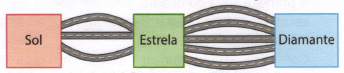
\includegraphics[width=1\linewidth]{6FMA112_imagens/imagem1}
			\begin{enumerate}[a)]
				\item Quantos caminhos são possíveis para ir da cidade Sol até a cidade Diamante? \\\\\\\\\\\\\\\\\\\\\\\\
				\item Quantos caminhos são possíveis para a família Toledo ir e voltar de viagem, passando pela cidade Estrela na ida e na volta? \\\\\\\\\\\\\\
			\end{enumerate}
			\item Um palhaço utiliza um figurino com 4 peças: uma peruca, um chapéu, um macacão e um par de sapatos. Em seu guarda-roupa há 5 perucas, 2 chapéus, 6 macacões e 3 pares de sapatos. \\ 
			De quantos modos diferentes ele pode se vestir para suas apresentações? \newpage
			\item Uma marca de relógios lançou um modelo que permite combinar pulseiras, aros e caixas de diferentes cores. O conjunto é composto por 6 pulseiras, 4 aros e caixas de diferentes cores. No desenho a seguir, temos a pulseira azul em três composições distintas, uma com o aro preto e a caixa branca, outra com o aro azul e a caixa preta e a outra com o aro branco e a caixa cinza. \\
			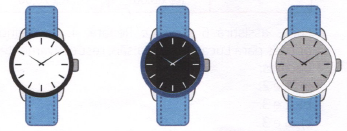
\includegraphics[width=1\linewidth]{6FMA112_imagens/imagem2}
			Qual é o número de composições possíveis usando todas as 13 peças desse modelo de relógio? \\\\\\\\\\\\\\\\\\\\\\\\\\\\\\\\\\\\\\\\\\
			\item Bruno pegou o mapa de sua cidade com as divisões dos bairros, como representado abaixo. Ele só tem disponíveis lápis de 4 cores diferentes e resolveu colorir cada bairro com uma cor, podendo repeti-las no mapa, contanto que os bairros pintados da mesma cor não seja adjacentes. \\
			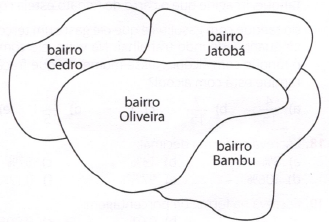
\includegraphics[width=1\linewidth]{6FMA112_imagens/imagem3}
			De quantas formas distintas Bruno pode colorir esse mapa?
		\end{enumerate}
		$~$ \\ $~$ \\ $~$ \\ $~$ \\ $~$ \\ $~$ \\ $~$ \\ $~$ \\ $~$ \\ $~$ \\ $~$ \\ $~$ \\ $~$ \\ $~$ \\ $~$ \\ $~$ \\ $~$ \\ $~$ \\ $~$ \\ $~$ \\ $~$ \\ $~$
	\end{multicols}
\end{document}